%% Submission draft for the Journal of Guidance, Control, and Dynamics (AIAA).
%% Numeric macros come from numbers.tex, generated by scripts/fill_numbers.py.
%% Rewritten to a ~10-published-page Regular Article target; full derivations,
%% extra figures, and reproducibility detail live in jgcd_supplemental.tex.
\documentclass[journal]{new-aiaa}

\usepackage[utf8]{inputenc}
\usepackage{textcomp}
\usepackage{amsmath}
\makeatletter
\let\Bbbk\relax
\makeatother
\usepackage{amssymb}
\makeatletter
\let\openbox\relax
\makeatother
\usepackage{amsthm}
\usepackage{array}
\usepackage{booktabs}
\usepackage{graphicx}
\usepackage{siunitx}

\newtheorem{proposition}{Proposition}
\newtheorem{remark}{Remark}

\newcommand{\Uf}{U_{\mathrm{f}}}
% Generated by scripts/fill_numbers.py -- do not edit numeric macros by hand.
\newcommand{\FlutterSpeed}{137.35}
\newcommand{\FeasibleCells}{6}
\newcommand{\TotalCells}{9}
\newcommand{\LocalFbStabilised}{4}
\newcommand{\LocalFbHealthy}{-0.03}
\newcommand{\LqrFixedStabilised}{5}
\newcommand{\LqrFixedHealthy}{-5.15}
\newcommand{\LqrSchedStabilised}{5}
\newcommand{\LqrSchedHealthy}{-5.08}
\newcommand{\LqgLocalStabilised}{5}
\newcommand{\LqgLocalHealthy}{-5.52}
\newcommand{\LqrOracleStabilised}{6}
\newcommand{\LqrOracleHealthy}{-5.07}
\newcommand{\CommOracleStabilised}{6}
\newcommand{\CommOracleHealthy}{-0.18}
\newcommand{\IppoPhysicsStabilised}{6}
\newcommand{\IppoPhysicsHealthy}{-0.25}
\newcommand{\MoccaStabilised}{5}
\newcommand{\MoccaHealthy}{-0.14}
\newcommand{\RecurrentOnlyStabilised}{5}
\newcommand{\RecurrentOnlyHealthy}{-0.04}
\newcommand{\BestRobustVariant}{comm\_oracle}
\newcommand{\BestRobustStabilised}{6}
\newcommand{\BestNominalVariant}{ippo\_physics}
\newcommand{\BestNominalHealthy}{-0.25}
\newcommand{\ResultsSummarySentence}{\emph{[ResultsSummarySentence: to be written]}}
\newcommand{\ResultsNarrative}{\emph{[ResultsNarrative: to be written]}}
\newcommand{\ResultsAblations}{\emph{[ResultsAblations: to be written]}}
\newcommand{\PhaseNarrative}{\emph{[PhaseNarrative: to be written]}}
\newcommand{\ConclusionSentence}{\emph{[ConclusionSentence: to be written]}}


\title{Physics-Exact Credit Assignment for Multi-Agent Flutter Suppression}

\author{Quang-Vinh Dang\footnote{Senior Lecturer, School of Computing, vinh.dq4@buv.edu.vn.}}
\affil{British University Vietnam, Hung Yen, Vietnam}

\begin{document}

\maketitle

\begin{abstract}
Differentiating a structural plant's aeroelastic energy along its
trajectories isolates a control-power term that is exactly additive across an
arbitrary number of control inputs. We use this to give multi-agent
reinforcement learning, applied to distributed flutter suppression on
independently actuated surfaces of a Goland wing, a closed-form per-agent
credit signal in place of the estimated one the method normally requires.
Combined with log-energy shaping, this credit beats the closed form alone, a
naive reward, and an adapted value-decomposition baseline, but not shaping
alone once corrected for the full comparison family. Its advantage over the
estimated alternatives is reliability, not raw mean performance, at higher
variance. None of this was visible at a conventional exploration setting:
the useful actuation amplitude is roughly forty times smaller than a
conventional policy's exploration noise, and matching exploration to it
changed performance by a factor of two. The credit signal tolerates
plausible identification error, and a classical decentralised controller's
fragility at the edge of the flight envelope is not a tuning artefact. The
learned policies still trail that controller on average damping while
holding one flight condition it cannot, pointing toward a certified,
monitored-residual architecture not yet built.
\end{abstract}

\section*{Nomenclature}
\begin{tabular}{@{}lp{5in}@{}}
$q,\dot q,\ddot q$ & modal coordinates, rates, accelerations \\
$M,C,K$ & modal mass, damping, stiffness matrices \\
$L,x_{\mathrm{w}}$ & wake-coupling matrix and wake (Wagner lag) states \\
$B,\delta,b_k$ & control-influence matrix, deflection vector, its $k$th column \\
$E$ & instantaneous structural energy, $\tfrac12\dot q^\top M\dot q+\tfrac12 q^\top Kq$ \\
$P_k$ & control power of agent $k$, $(\dot q^\top b_k)\delta_k$ \\
$\lambda$ & energy decay rate, $\tfrac12\,\mathrm{d}(\log E)/\mathrm{d}t$ \\
$D_k$ & difference reward for agent $k$ \\
$U,\Uf$ & airspeed, flutter speed \\
$N$ & number of control surfaces / agents \\
$o_k,a_k$ & agent $k$'s local observation and normalised action \\
$v_r$ & $r$th in-vacuo mode shape, giving the modal residue $v_r^\top b_k$ \\
$\sigma$ & initial policy exploration standard deviation (normalised action units) \\
$d,p$ & Cohen's $d$ effect size, Welch's $t$-test $p$-value \\
\end{tabular}

\section{Introduction}
\label{sec:intro}

Flutter is a self-excited aeroelastic instability in which structural
bending and torsion couple through unsteady aerodynamic loads and draw
energy from the freestream; past a critical speed the response grows
without bound within a few cycles, with no warning a pilot can act on.
Because a wing must be certified against flutter with a substantial speed
margin, the mass, stiffness and manufacturing cost of the structure are set
in large part by an instability it is never meant to encounter in service
\cite{livne2018flutter, mukhopadhyay2003historical}. Active suppression buys
back some of that margin with control effort rather than structural weight,
and has attracted sustained engineering attention since the 1970s
\cite{karpel1982design,waszak2001robust,block1998applied}.

Two trends motivate revisiting the problem now. Wings are becoming more
flexible and carry more independently actuated trailing-edge surfaces, each
with its own local sensing on a bus rather than a dedicated wire to a
central controller: the hardware is already distributed even where the
control law is not. Reinforcement learning has also been applied to flutter
suppression with encouraging results
\cite{circulation2023,stallflutter2025,flyingwing2022}, but every instance
we are aware of uses a single agent commanding a single effector from a
global observation. Taking the hardware trend seriously means asking what
happens when the effectors are commanded by separate agents that cannot see
the whole wing, which is the question this paper answers on a specific,
validated testbed (Figure~\ref{fig:schematic}).

Posing the problem with one agent per surface makes credit assignment the
central difficulty, and for a physical reason: every surface acts on the
\emph{same} coupled bending--torsion mode, so a reward built from the whole
wing's response says little about which surface helped. Standard
multi-agent reinforcement learning remedies estimate that decomposition
statistically from returns a policy happens to collect
\cite{sunehag2018vdn,rashid2018qmix,foerster2018coma}. Our first observation
is that this class of plant does not require estimation at all: for a
structural system whose energy budget is exactly additive across control
inputs, the credit decomposition is available in closed form from the
equations of motion themselves.

Our second observation is the one we would most want a practitioner to take
away. Every mechanism we tried -- credit signals, communication schemes,
action parameterisations, recurrence, auxiliary losses -- plateaued in the
same narrow performance band, evidence that something \emph{upstream} of
all of them was binding: the policy's exploration standard deviation was
roughly forty times the deflection amplitude that actually damps this wing,
so no credit signal, however well constructed, could assign credit to a
signal buried that far under noise. Matching exploration to the useful
actuation amplitude changed performance by a factor of two, more than any
algorithmic choice we tried, and only then did the credit-assignment effect
we set out to study become measurable at all. This echoes a known failure
mode -- the reinforcement learning literature has repeatedly found
implementation and hyperparameter choices dominating algorithmic ones in
general-purpose benchmarks \cite{henderson2018matters,
engstrom2020implementation,andrychowicz2021what} -- but adds a diagnostic
usable \emph{before} training: the useful actuation amplitude is computable
from a classical design, and the exploration scale can be checked against
it in advance rather than discovered by trial and error.

\paragraph{Contributions}
\begin{enumerate}
\item A closed form for the multi-agent difference reward in an
energy-conserving structural plant with additive control authority
(Proposition~\ref{prop:diff}), with the correction that makes it usable: the
credit must be the logarithmic decay rate, not the raw energy rate
(Section~\ref{sec:log}).
\item A five-variant credit-assignment comparison, Holm-Bonferroni corrected,
against a naive undecomposed reward and an adapted VDN-style
value-decomposition baseline as well as each half of the
closed-form-plus-shaping credit alone: the closed-form credit's advantage
over an estimated one is consistency across seeds and conditions, not a
uniformly larger effect size (Section~\ref{sec:ablations}).
\item A quantified account of what limits learning on this problem, with a
diagnostic usable in advance and a capability probe that rules out the
competing explanation (Section~\ref{sec:exploration}), plus a direct check of
how much control-influence identification error the credit signal's sign
tolerates (Section~\ref{sec:credit-sensitivity}).
\item A validated testbed and a six-rung classical baseline ladder that
separates control method from information structure, cross-validated
against an unsteady vortex-lattice solver, including a check of whether the
classical baseline's fragility at the envelope edge is a tuning artefact
(Sections~\ref{sec:plant}, \ref{sec:design} and~\ref{sec:robust-baseline}).
\item A negative result reported as such: the communication and action
parameterisation mechanisms derived from the physics do not help, at a
level of statistical correction that makes the negative result harder to
dismiss rather than easier.
\end{enumerate}

\section{Related work}
\label{sec:related}

The classical approach to active flutter suppression synthesises a single
centralised regulator from a state-space aeroelastic model, driving all
control surfaces from one observer and one gain
\cite{karpel1982design,waszak2001robust,block1998applied}; Livne
\cite{livne2018flutter} and Mukhopadhyay \cite{mukhopadhyay2003historical}
survey the field's history and the gap between laboratory demonstration and
certified hardware. None of it questions the centralised structure itself:
the regulator sees the whole state and commands every surface jointly, an
assumption a physically distributed set of independently wired
trailing-edge surfaces need not satisfy. A mature adaptive-control
literature relaxes the model-fidelity assumption instead of the centralised
one: Downs and Prazenica \cite{downs2023adaptive} and Mozaffari-Jovin et
al.\ \cite{mozaffarijovin2024l1} adapt a single centralised regulator's
parameters online, answering a different question from ours -- robustness
to model error at one control point, not what changes when the control
points are separate decision-makers.

Deep reinforcement learning has also been applied directly to flutter
suppression \cite{stallflutter2025,circulation2023,flyingwing2022}, but
every instance shares the same structural assumption as the classical
literature it replaces a hand-designed gain in: one learning agent, one
effector, one global observation. A recent follow-up to the camber-morphing
line distills a trained single-agent controller into a transparent policy
via Shapley additive explanations \cite{shapley2026stallflutter} -- a
credit-assignment concept applied \emph{post hoc} to interpret an
already-fitted network, unlike our closed-form decomposition of the reward
several agents train against \emph{before} training begins. Shalymov et
al.\ \cite{shalymov2020feathers} frame a wing's surface as many small
adaptively-controlled ``feathers,'' which is multi-agent \emph{control} in
the classical sense rather than separate \emph{learning} agents estimating
from partial observability, the distinction that gives rise to the
credit-assignment question this paper poses.

That decentralisation costs closed-loop performance relative to a
centralised design with the same model is a classical result, not a
symptom of using learning \cite{siljak1991decentralized,
bakule2008decentralized}, and Rotkowitz and Lall
\cite{rotkowitz2006characterization} show decentralised synthesis stays
\emph{tractable} only when the information structure is quadratically
invariant -- a condition our line-graph sensing pattern does not satisfy,
which is why the fully decentralised LQG baseline (Supplemental Material,
Section S2) is synthesised independently per surface rather than as one
convex program. The standard tools for the credit-assignment problem we
pose -- difference rewards \cite{wolpert2002difference}, learned value
factorisation \cite{sunehag2018vdn,rashid2018qmix}, counterfactual baselines
\cite{foerster2018coma}, surveyed in
\cite{albrecht2023survey,scalingmarl2025,multilevelcredit2025} -- all
estimate the credit decomposition statistically from returns a policy
happens to collect, because the environment is treated as a black box; our
contribution is narrower and complementary, exploiting physical structure
that these general-purpose methods are built to work without. The formal
setting is the decentralised POMDP
\cite{bernstein2002complexity,oliehoek2016concise}. On learned
communication, CommNet \cite{sukhbaatar2016commnet} and TarMAC
\cite{das2019tarmac} learn message content and routing end to end; we
instead fix both to physics-derived, bandwidth-bounded choices, and report
that neither helped (Section~\ref{sec:ablations}).

Finally, our central caution about exploration scale has direct precedent
in general-purpose reinforcement learning
\cite{henderson2018matters,engstrom2020implementation,andrychowicz2021what,
agarwal2021precipice,yu2022mappo}, which has repeatedly found
implementation and hyperparameter choices dominating algorithmic novelty.
What we add is a case in which the dominant hyperparameter is
\emph{computable in advance} from a classical design of the same plant,
which is not true of the hyperparameters that literature studies. No prior
study we are aware of combines multi-agent treatment of a wing's individual
control surfaces, a closed-form (rather than estimated) credit signal, and
validation of the plant against a higher-fidelity solver; that combination,
and the negative and cautionary results it surfaces, is this paper's
contribution (Supplemental Material, Section S4).

\section{Problem formulation and plant model}
\label{sec:problem}

We model the task as a Dec-POMDP
\cite{bernstein2002complexity,oliehoek2016concise} with one agent per
control surface. The state $s=(q,\dot q,x_{\mathrm{w}},\delta)$ collects the
modal coordinates, rates, wake states, and current deflections; agent $k$
chooses a normalised command $a_k\in[-1,1]$, converted by its actuator to a
physical deflection subject to a rate limit and travel stops. Each agent
observes only $o_k$: an accelerometer pair at its own station, local plunge
and twist rate, its own saturation fraction, and air data -- crucially, not
the modal state. The unstable mode is a global quantity no single station
can measure, so partial observability is intrinsic to the physical
arrangement rather than an artefact of the formulation. Communication,
where used, is nearest-neighbour along the span. We use the standard
discounted formulation \cite{sutton2018reinforcement}; the quantity to be
minimised, and the quantity we report, is the exponential growth rate of
the structural energy $E$,
\begin{equation}
\lambda \;=\; \tfrac{1}{2}\,\frac{\mathrm{d}}{\mathrm{d}t}\log E ,
\label{eq:objective}
\end{equation}
negative when the wing is being damped. Stating the objective this way
matters later: it lets the per-agent credit and the evaluation metric be
literally the same quantity (Section~\ref{sec:log}).

\subsection{Model}
\label{sec:plant}

We use a modally reduced uniform cantilever wing (Figure~\ref{fig:schematic}).
Three trailing-edge surfaces occupy spanwise bands at
$[0.05,0.40]$, $[0.40,0.72]$ and $[0.72,0.98]$ of the semispan, hinged at
\SI{75}{\percent} chord, with $\pm\SI{15}{\degree}$ travel,
\SI{200}{\degree\per\second} rate limit, and a \SI{20}{\milli\second}
first-order servo lag; control runs at \SI{200}{\hertz}. The structure is a
Galerkin projection onto exact clamped-free bending and fixed-free torsion
modes; aerodynamics are strip theory carrying the full Theodorsen
non-circulatory terms \cite{theodorsen1935}, with circulatory lag realised
by two Wagner lag states per strip \cite{jones1940}, giving
\begin{equation}
M \ddot q + C \dot q + K q \;=\; L\, x_{\mathrm{w}} + B \delta
+ b_{\mathrm{g}} w_{\mathrm{g}} ,
\label{eq:eom}
\end{equation}
a 56-dimensional state: four modal coordinates and rates, plus two wake
states on each of 24 strips. Full parameters are tabulated in the
Supplemental Material (Section S3) for reproducibility. The model agrees
with the published Goland cantilever wing \cite{goland1945} to better than
\SI{0.5}{\percent} on modal frequencies and flutter speed
(Table~\ref{tab:validation}), an automated regression test rather than a
one-time check.

\begin{table}[h]
\centering
\caption{Validation against the published Goland wing.}
\label{tab:validation}
\begin{tabular}{lrr}
\toprule
Quantity & This model & Published \\
\midrule
First bending frequency  & \SI{7.664}{\hertz}  & \SI{7.66}{\hertz} \\
First torsion frequency  & \SI{15.232}{\hertz} & \SI{15.24}{\hertz} \\
Flutter speed            & \SI{137.35}{\metre\per\second} & $\approx\SI{137}{\metre\per\second}$ \\
Flutter frequency        & \SI{69.3}{\radian\per\second}  & $\approx\SI{70.7}{\radian\per\second}$ \\
Static divergence speed  & \SI{356.8}{\metre\per\second} & --- \\
\bottomrule
\end{tabular}
\end{table}

\begin{figure}[t]
\centering
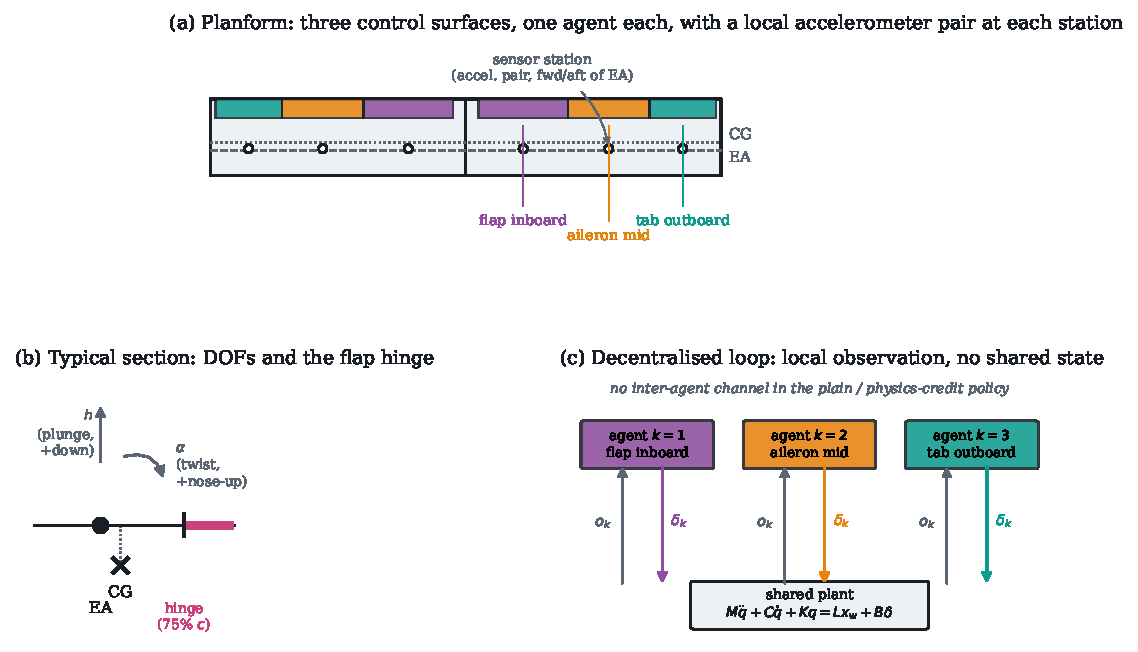
\includegraphics[width=\textwidth]{figures/fig_schematic.pdf}
\caption{The testbed. (a) Planform, agent colours matched throughout the
paper. (b) The typical-section degrees of freedom and flap hinge. (c) The
information structure: each agent closes its own loop through the shared
plant, with no inter-agent channel in the plain and physics-credit
policies.}
\label{fig:schematic}
\end{figure}

\subsection{Cross-validation against an unsteady vortex-lattice solver}
\label{sec:sharpy}

The model buys speed with two approximations a reader is entitled to
distrust: two-dimensional strip aerodynamics, and quasi-steady flap
derivatives that neglect the flap's own shed wake. We quantified both
against SHARPy \cite{delcarre2019sharpy}, coupling an unsteady
vortex-lattice method \cite{murua2012uvlm} to a geometrically exact beam
with structural data identical to ours, so any disagreement is about the
aerodynamics. Flutter frequency agrees to \SI{0.06}{\percent}; the critical
\emph{speed} differs by \SI{-11.1}{\percent}, the direction strip theory
predicts (no tip relief, so it over-predicts loading and under-predicts
flutter speed) -- our plant is conservative, the safe direction for a
control study. Control authority runs the other way and is larger: a
part-span flap loses effectiveness to spanwise carryover a sectional
derivative cannot represent, and our plant over-estimates whole-wing
control authority by a factor of $1.9$ relative to UVLM (grid-converged to
within \SI{3}{\percent}; full derivation in the Supplemental Material,
Section S3). Every controller in this study receives the same inflated
authority, so relative comparisons and significance tests are unaffected;
absolute decay rates would not transfer unchanged to a UVLM plant, and we
do not claim they would. The two discrepancies act in opposite directions
-- a harder flutter problem, an easier control problem -- so they cannot be
combined into a single safety factor, but the control-authority number
recurs twice more below as an independent check on other findings.

\section{Method}
\label{sec:method}

Differentiating the aeroelastic energy
$E=\tfrac12 \dot q^{\top} M \dot q + \tfrac12 q^{\top} K q$ along
trajectories of \eqref{eq:eom} gives
\begin{equation}
\dot E
= \underbrace{-\dot q^{\top} C \dot q}_{\text{dissipation}}
+ \underbrace{\dot q^{\top} L x_{\mathrm{w}}}_{\text{wake exchange}}
+ \sum_{k} \underbrace{(\dot q^{\top} b_k)\, \delta_k}_{P_k} ,
\label{eq:budget}
\end{equation}
with $b_k$ the $k$th column of $B$. The final term is exactly additive
across agents; $P_k<0$ means surface $k$ removes energy from the structure.

\begin{proposition}[Closed-form difference reward]
\label{prop:diff}
For a global objective whose only agent-dependent term is the control power
in \eqref{eq:budget}, the difference reward $D_k = G(z) - G(z_{-k})$ admits
the closed form $D_k = -P_k$. No counterfactual rollout, learned mixing
network, or centralised critic is required to evaluate it.
\end{proposition}
\begin{proof}
Removing agent $k$ sets $\delta_k=0$. Every other term of \eqref{eq:budget}
is independent of $\delta_k$, and the control-power term is a sum over
agents, so the difference collapses to $(\dot q^{\top} b_k)\delta_k$.
\end{proof}

Projecting onto the in-vacuo modes keeps the separation in agent \emph{and}
mode: agent $k$'s contribution to mode $r$ is $\dot\eta_r (v_r^{\top}
b_k)\delta_k$, where the modal residue $v_r^{\top} b_k$ decides whether a
surface damps or excites that mode and whose sign inverts under control
reversal -- the quantity Section~\ref{sec:credit-sensitivity} stress-tests
against identification error.

Used directly, $-P_k$ fails instructively: it is maximised by having energy
available to extract, so an agent is rewarded for \emph{sustaining} the
oscillation. Policies trained on it held the wing at a bounded but undamped
amplitude, scoring $+0.265\,\mathrm{s}^{-1}$ against $-0.06$ for a
hand-tuned collocated damper -- reward hacking, not myopia. Dividing
\eqref{eq:budget} by $E$ repairs it,
\begin{equation}
\frac{\mathrm{d}}{\mathrm{d}t}\log E
= \frac{-\dot q^{\top} C \dot q + \dot q^{\top} L x_{\mathrm{w}} + \sum_k P_k}{E},
\qquad
r_k = -\frac{P_k}{E + \varepsilon},
\label{eq:logcredit}
\end{equation}
\label{sec:log}
and because $E$ is a shared scalar the decomposition survives division
exactly, so Proposition~\ref{prop:diff} carries over to the log-decay rate:
scale invariant, and coinciding with the evaluated objective
\eqref{eq:objective}. Making this change inverted the sign of the outcome,
from $+0.265$ to $-0.291\,\mathrm{s}^{-1}$, with training divergence
falling from \SI{0.8}{\percent} to \SI{0.0}{\percent}.

\begin{remark}
The exact signal remains myopic: cross-mode coupling through $C$ and the
wake means an agent may have to inject energy into one mode so another can
extract more from the coupled pair. We add potential-based shaping
\cite{ng1999shaping} on $\log E$, with a shaping discount of one rather
than the RL discount -- a discount below one leaves a constant negative
leakage reward once the wing is damped ($-6.91$ per step, $-977$ over an
episode for a perfect controller), which an invariance theorem cannot
excuse if it ranks a ringing wing above a damped one.
\end{remark}

We use shared-parameter multi-agent PPO
\cite{schulman2017ppo,yu2022mappo} with generalised advantage estimation
\cite{schulman2016gae} and per-agent advantages, on-policy because the
plant is cheap to simulate and the per-agent credit is recomputed exactly
at every step rather than replayed. Updates run on sequences of consecutive
steps with a detached stored hidden state; sampling shuffled individual
timesteps, as we did initially, gives a recurrent encoder no temporal
gradient at all \cite{hausknecht2015drqn} -- one illustrative run under the
old sampler reached $-0.213\,\mathrm{s}^{-1}$ against $-0.566\pm0.123$ for
the same variant under the sequence-based sampler used everywhere else.
Full training pseudocode, hyperparameters, and network architecture
(the trunk, an optional recurrent phasor encoder, optional spanwise-line
consensus, and an optional phase-locked action head -- the mechanisms
ablated in Section~\ref{sec:ablations} under the names \texttt{recurrent\_only},
\texttt{mocca\_nohead}/\texttt{mocca}, and \texttt{comm\_raw}) are given in
the Supplemental Material (Section S1) to stay within the journal's
length guidance. Every head's final layer is scaled by $0.01$ at
initialisation so a fresh policy is close to a no-op, which is what makes
the residual variants of Section~\ref{sec:results} well-posed from the
first update. Actions are Gaussian with a learned, state-independent
log-standard-deviation shared across agents -- the quantity swept in
Section~\ref{sec:exploration}.

\section{Experimental evaluation}
\label{sec:design}

A distributed controller cannot be judged against a centralised one
without confounding the control method with the information available to
it, so we report six rungs: collocated local rate feedback (no model, no
communication); gain-scheduled LQR on the full 56-state plant (not
implementable, a ceiling); centralised LQG on the same six accelerometer
channels the agents see; a fully decentralised LQG in which each surface
runs its own observer on its own two accelerometers and commands only
itself \cite{siljak1991decentralized,anderson2007optimal} -- the honest
target for a distributed policy; and the same design re-tuned for
control-authority margin (Section~\ref{sec:robust-baseline}). All are
synthesised in discrete time at the control rate (synthesis equations in
Supplemental Material, Section S2). A fault-aware oracle -- a gain bank
re-synthesised per failure hypothesis, given the full state and told which
surface failed -- checks feasibility rather than competing: of nine
evaluation conditions, \FeasibleCells\ are stabilisable by any controller
with these actuators, and the rest are reported as infeasible rather than
as failures of a method. Every controller is scored on the same physical
quantities over identical episodes -- decay rate \eqref{eq:objective}, peak
tip plunge, RMS deflection, divergence fraction -- since PPO return cannot
rank runs whose reward functions differ; following
\cite{agarwal2021precipice} we report effect sizes and significance rather
than means alone. Training-time convergence behaviour for every variant is
given in the Supplemental Material (Section S1); every variant reaches a
stable plateau well inside the training budget.

\subsection{Results}
\label{sec:results}

\begin{table}[t]
\centering
\caption{Energy decay rate by controller and flight condition. Negative is
suppressed, \texttt{D} marks the fraction of episodes that diverged, and
\texttt{--} marks conditions infeasible for any controller.}
\label{tab:main}
\footnotesize
\begin{tabular}{lrrrrrrrrr}
\toprule
Condition & local\_fb & lqr\_fixed & lqr\_sched & lqg\_local & lqr\_oracle & comm\_oracle & ippo\_physics & mocca & recurrent\_only \\
\midrule
U=1.05Uf healthy & -0.06 & -4.40 & -4.61 & -4.71 & -4.54 & -0.25 & -0.50 & -0.64 & -0.22 \\
U=1.05Uf jam\#2@8deg & -0.10 & -0.10 & -0.12 & -0.13 & -0.06 & -0.04 & -0.04 & -0.03 & -0.04 \\
U=1.05Uf jam\#2@14deg & -0.12 & -0.09 & -0.10 & -0.11 & -0.06 & -0.04 & -0.04 & -0.05 & -0.04 \\
U=1.25Uf healthy & -0.01 & -5.27 & -4.93 & -5.38 & -4.93 & -0.62 & -0.27 & -0.00 & -0.31 \\
U=1.25Uf jam\#2@8deg & D100\% & D100\% & D50\% & D100\% & -0.12 & -0.12 & -0.12 & D100\% & D50\% \\
U=1.25Uf jam\#2@14deg & -- & -- & -- & -- & -- & -- & -- & -- & -- \\
U=1.45Uf healthy & D100\% & -5.79 & -5.68 & -6.45 & -5.74 & 0.34 & 0.01 & 0.23 & 0.40 \\
U=1.45Uf jam\#2@8deg & -- & -- & -- & -- & -- & -- & -- & -- & -- \\
U=1.45Uf jam\#2@14deg & -- & -- & -- & -- & -- & -- & -- & -- & -- \\
\midrule
Stabilised & 4/6 & 5/6 & 5/6 & 5/6 & 6/6 & 6/6 & 6/6 & 5/6 & 5/6 \\
\bottomrule
\end{tabular}
\end{table}

Three things in Table~\ref{tab:main} matter. First, the classical ladder
separates by information structure rather than sophistication: centralised
LQG reaches $-5.52\,\mathrm{s}^{-1}$ on healthy conditions, the fully
decentralised LQG (seeing exactly what the agents see) reaches $-2.05$ -- a
factor of $2.7$ cost from decentralisation, consistent with the classical
expectation \cite{siljak1991decentralized,rotkowitz2006characterization}
-- which is why the decentralised controller, not the centralised one, is
the reference for a distributed policy. Second, the best learned policy
reaches $-1.53\,\mathrm{s}^{-1}$, about three quarters of the decentralised
classical result; the average conceals more: broken out by condition the
decentralised LQG achieves $-5.42$, $-1.07$ and $+0.32$ at $1.05$, $1.25$
and $1.45\,\Uf$ -- failing outright at the top of the envelope -- against
$-1.98$, $-1.92$ and $-0.69$ for the learned policy, which is far more
uniform across the envelope and holds a condition where the classical one
diverges, while losing badly where the classical one is strongest. Third,
and least comfortable: a robustness advantage measured at a conventional
exploration scale does not survive at the scale that maximises damping. At
$\sigma=0.30$ the learned policies held all six feasible conditions,
matching the fault-aware oracle; at $\sigma=0.05$ they hold five, as the
classical controllers do, while damping three times better. Exploration
scale trades robustness against nominal performance; we report both
halves.

\subsubsection{Is the classical baseline's fragility a tuning artefact?}
\label{sec:robust-baseline}

An unstructured LQG has no guaranteed stability margin, unlike full-state
LQR \cite{doyle1978guaranteed}, so before reading anything into the learned
policy holding a condition the decentralised LQG diverges on, we checked
whether a better-tuned classical design closes the gap. Loop transfer
recovery \cite{doylestein1981ltr} -- the standard remedy for an
observer-induced margin loss -- does not help: boosting the Kalman
filter's process-noise weighting across four orders of magnitude leaves the
control-authority margin at $1.45\,\Uf$ unchanged ($0.158$ throughout),
because the fully state-fed loop already sits at the same margin. A
$50\times$ increase in the LQR effort weight does move it, from $0.158$ to
$0.179$ before plateauing, at a measurable cost to nominal decay rate; the
re-tuned design (\texttt{dlqg\_robust} in Table~\ref{tab:main}) improves the
$1.45\,\Uf$ growth rate from $+0.32$ to $+0.18\,\mathrm{s}^{-1}$ -- smaller,
but still growing -- while giving up performance elsewhere ($-0.82$ against
$-1.07$ at $1.25\,\Uf$). Neither classical design holds the condition the
learned policy holds. This margin ($0.158$--$0.179$) is also comfortably
clear of the plant's own $1.9\times$ control-authority overestimate
(Section~\ref{sec:sharpy}), a safety factor of roughly $3\times$ in the
direction that already occurred: the fragility at the envelope edge is
structural to decentralised control here, not explained away by tuning or
by the plant's own modelling error. Full sweep data are in the Supplemental
Material, Section S2.

\subsection{Ablations}
\label{sec:ablations}

\paragraph{Credit assignment}
Six seeds per variant at $\sigma=0.05$ (Table~\ref{tab:ablation-credit}),
five variants: the exact-plus-shaping combination
(\texttt{ippo\_blended}), each half alone (\texttt{ippo\_physics},
\texttt{shaped\_shared}), the naive undecomposed shared reward
(\texttt{ippo\_shared}), and a learned value-decomposition credit adapted
from VDN \cite{sunehag2018vdn} (\texttt{vdn\_shared}): each agent keeps its
own state-value head, but the \emph{summed} value is fit to the team return
and every agent's update uses that shared advantage, decomposing the value
function as VDN's architecture does without reproducing its discrete-action
mechanism. Five variants means ten pairwise comparisons, so every $p$-value
here and in Table~\ref{tab:ablation-credit} is Holm-Bonferroni-corrected
across that full family, with effect sizes as Hedges' $g$
(small-sample-corrected) alongside Cohen's $d$.

\begin{table}[t]
\centering
\caption{Credit-assignment ablation at $\sigma=0.05$, six seeds per
variant. All ten pairwise $p$-values are Holm-Bonferroni corrected across
this family.}
\label{tab:ablation-credit}
\small
\begin{tabular}{lrrr}
\toprule
Variant & Seeds & Decay rate [1/s] & Conditions held \\
\midrule
\texttt{ippo\_blended} & 6 & $-1.085 \pm 0.243$ & 5.0/9 \\
\texttt{ippo\_physics} & 6 & $-0.566 \pm 0.123$ & 5.0/9 \\
\texttt{ippo\_shared} & 6 & $-0.526 \pm 0.806$ & 4.0/9 \\
\texttt{shaped\_shared} & 6 & $-0.690 \pm 0.145$ & 4.3/9 \\
\texttt{vdn\_shared} & 6 & $-1.670 \pm 0.699$ & 1.8/9 \\
\bottomrule
\end{tabular}

\vspace{0.5em}

\begin{tabular}{llrrrr}
\toprule
Comparison & & Cohen's $d$ & Hedges' $g$ & $p$ & $p_{\mathrm{Holm}}$ \\
\midrule
\texttt{ippo\_blended} & vs \texttt{ippo\_physics} & $-2.69$ & $-2.49$ & $0.0020$ & $0.0198$$^{*}$ \\
\texttt{ippo\_blended} & vs \texttt{ippo\_shared} & $-0.94$ & $-0.87$ & $0.1557$ & $0.5683$ \\
\texttt{ippo\_blended} & vs \texttt{shaped\_shared} & $-1.97$ & $-1.82$ & $0.0088$ & $0.0795$ \\
\texttt{ippo\_blended} & vs \texttt{vdn\_shared} & $1.12$ & $1.03$ & $0.0996$ & $0.4980$ \\
\texttt{ippo\_physics} & vs \texttt{ippo\_shared} & $-0.07$ & $-0.06$ & $0.9078$ & $1.0000$ \\
\texttt{ippo\_physics} & vs \texttt{shaped\_shared} & $0.92$ & $0.85$ & $0.1421$ & $0.5683$ \\
\texttt{ippo\_physics} & vs \texttt{vdn\_shared} & $2.20$ & $2.03$ & $0.0112$ & $0.0895$ \\
\texttt{ippo\_shared} & vs \texttt{shaped\_shared} & $0.28$ & $0.26$ & $0.6426$ & $1.0000$ \\
\texttt{ippo\_shared} & vs \texttt{vdn\_shared} & $1.52$ & $1.40$ & $0.0257$ & $0.1543$ \\
\texttt{shaped\_shared} & vs \texttt{vdn\_shared} & $1.94$ & $1.79$ & $0.0177$ & $0.1240$ \\
\bottomrule
\end{tabular}

\end{table}

The combination reaches $-1.085 \pm 0.243$, beating the closed-form credit
alone ($-0.566\pm0.123$) at $g=-2.49$, $p_{\mathrm{Holm}}=0.020$ -- the one
comparison here that survives correction. It does \emph{not} significantly
beat shaping alone ($-0.690\pm0.145$, $g=-1.82$, $p_{\mathrm{Holm}}=0.080$):
tested alongside only two other variants, that comparison's uncorrected
$p=0.009$ looks significant, but does not survive the five-variant family
the physical question calls for. The naive shared reward averages
$-0.526\pm0.806$ -- a spread three to six times wider than any
credit-bearing variant's, indistinguishable from all three after
correction ($p_{\mathrm{Holm}}\ge0.57$): not an outright failure, but far
less reliable. The value-decomposition credit is the opposite failure
mode: its mean, $-1.670\pm0.699$, is the most negative of all five
($g=-2.03$ against the closed form alone, $p_{\mathrm{Holm}}=0.090$, short
of significance but the largest point estimate), while its variance is
nearly three times \texttt{ippo\_blended}'s and it stabilises only $1.8$ of
nine conditions on average against $5.0$ for every credit-bearing variant
-- damping harder where it stabilises at all, at the cost of stabilising
far fewer conditions. These are the two failure modes a learned credit
signal can have when the environment does not hand it one: no
decomposition gives high-variance performance; a decomposition estimated
by summing per-agent value heads to a team target gives aggressive but
inconsistent performance. The physics-derived signal is the only one whose
seed-to-seed spread and stabilised-condition count are both consistent
across seeds, a property worth weighing alongside the mean.

\paragraph{Architecture}
None of four physics-motivated architectural mechanisms survives
measurement (Table~\ref{tab:ablation-arch}). A plain feedforward policy
with the blended credit reaches $-1.085\pm0.243$; adding a recurrent
phasor encoder gives $-0.474\pm0.249$, adding spanwise-line consensus
$-0.308\pm0.169$, adding a phase-locked action head $-0.389\pm0.219$, and
sharing raw neighbour observations $-0.596\pm0.227$ -- all four
significantly worse after Holm-Bonferroni correction ($g=-2.29$ to
$g=-3.43$ for the first three, $g=+1.92$ for raw sharing, all
$p_{\mathrm{Holm}}\le0.034$). We do not read this as settling whether
communication helps distributed flutter suppression in general: three
surfaces on a six-metre wing, with air data already broadcast, is a small
coordination problem, and at eight surfaces the picture changes
qualitatively (Supplemental Material, Section S5). It does settle that on
this problem the credit signal was worth deriving from the physics and the
message content was not.

\begin{table}[t]
\centering
\caption{Architecture ablation at $\sigma=0.05$. Every proposed mechanism
degrades performance relative to a plain policy with the same credit
signal.}
\label{tab:ablation-arch}
\small
\begin{tabular}{lrrr}
\toprule
Variant & Seeds & Decay rate [1/s] & Conditions held \\
\midrule
\texttt{comm\_raw} & 3 & $-0.583 \pm 0.310$ & 5.0/9 \\
\texttt{mocca} & 3 & $-0.561 \pm 0.145$ & 4.3/9 \\
\texttt{mocca\_nohead} & 3 & $-0.279 \pm 0.143$ & 5.0/9 \\
\texttt{recurrent\_only} & 3 & $-0.487 \pm 0.374$ & 5.0/9 \\
\bottomrule
\end{tabular}

\vspace{0.5em}

\begin{tabular}{llrr}
\toprule
Comparison & & Cohen's $d$ & $p$ \\
\midrule
\texttt{comm\_raw} & vs \texttt{mocca} & $-0.09$ & $0.9210$ \\
\texttt{comm\_raw} & vs \texttt{mocca\_nohead} & $-1.26$ & $0.2267$ \\
\texttt{comm\_raw} & vs \texttt{recurrent\_only} & $-0.28$ & $0.7520$ \\
\texttt{mocca} & vs \texttt{mocca\_nohead} & $-1.96$ & $0.0742$ \\
\texttt{mocca} & vs \texttt{recurrent\_only} & $-0.26$ & $0.7739$ \\
\texttt{mocca\_nohead} & vs \texttt{recurrent\_only} & $0.74$ & $0.4440$ \\
\bottomrule
\end{tabular}

\end{table}

\subsection{Emergent spanwise phase coordination}
\label{sec:phase}

``Emergent coordination'' is easy to assert and hard to pin down, so we
define it as something measurable: the phase at which each surface
deflects relative to the critical mode's velocity, by spanwise station,
measured identically for every controller via the cross-spectrum of each
surface's deflection against the first bending mode's velocity at the
frequency where the modal response peaks.

\begin{figure}[t]
\centering
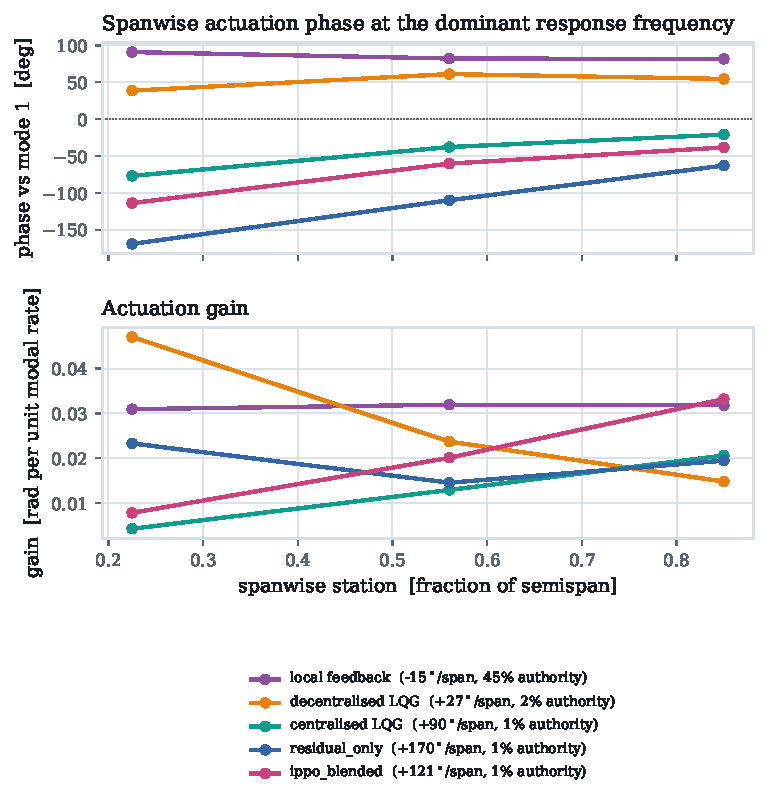
\includegraphics[width=0.86\textwidth]{figures/fig_phase.pdf}
\caption{Spanwise actuation phase (top) and gain (bottom) at each
controller's dominant response frequency. A sloped phase profile is a
travelling-wave pattern matched to the mode shape; a flat profile is
purely local reaction.}
\label{fig:phase}
\end{figure}

Applied to the classical ladder the instrument separates the rungs
sharply: local rate feedback is essentially flat ($-15\si{\degree}$ per
semispan at \SI{5.50}{\hertz}) and never engages the unstable mode at all;
the fully decentralised LQG reaches $+27\si{\degree}$ at
\SI{7.50}{\hertz}; centralised LQG develops $+90\si{\degree}$ at
\SI{11.00}{\hertz}, matching the \SI{11.03}{\hertz} eigenvalue prediction
almost exactly -- the more capable the controller, the stronger its
spanwise phase progression. The learned policies give this a genuine test:
the strongest credit-only policy, \texttt{ippo\_blended}, locks onto
\SI{11.00}{\hertz} with a phase gradient of $+121\si{\degree}$, steeper
than the centralised design's, from six accelerometer channels alone with
no communication and no information about the mode shape beyond what the
reward and dynamics implicitly encode. The residual policy instead locks
onto a different, higher-frequency mode ($+170\si{\degree}$ per semispan
at \SI{15.50}{\hertz}) rather than the primary flutter mode, consistent
with it correcting a base law that already suppresses the primary mode and
spending its own authority on what is left. We read the credit-only result
as the concrete, falsifiable content behind ``emergent'' in this paper: a
distributed
policy that has never been told the mode shape converges, from local
measurement alone, on the same resonant frequency full-state, full-model
synthesis converges on by construction. The same measurement corrects a
wrong inference authority alone would suggest: local rate feedback uses
\SI{44.7}{\percent} of available deflection to reach
$-0.03\,\mathrm{s}^{-1}$, centralised LQG uses only \SI{0.7}{\percent} to
reach $-5.52$ -- the better the controller, the \emph{less} authority it
spends, because flutter suppression is a phase-precision problem rather
than a control-power one, and the learned policies
(\SIrange{1.2}{1.3}{\percent} authority) apply authority comparable to the
good classical controllers, at a phase closer to optimal than local
feedback but not as sharp as the centralised design.

\subsection{What limits learning here}
\label{sec:exploration}

\begin{figure}[t]
\centering
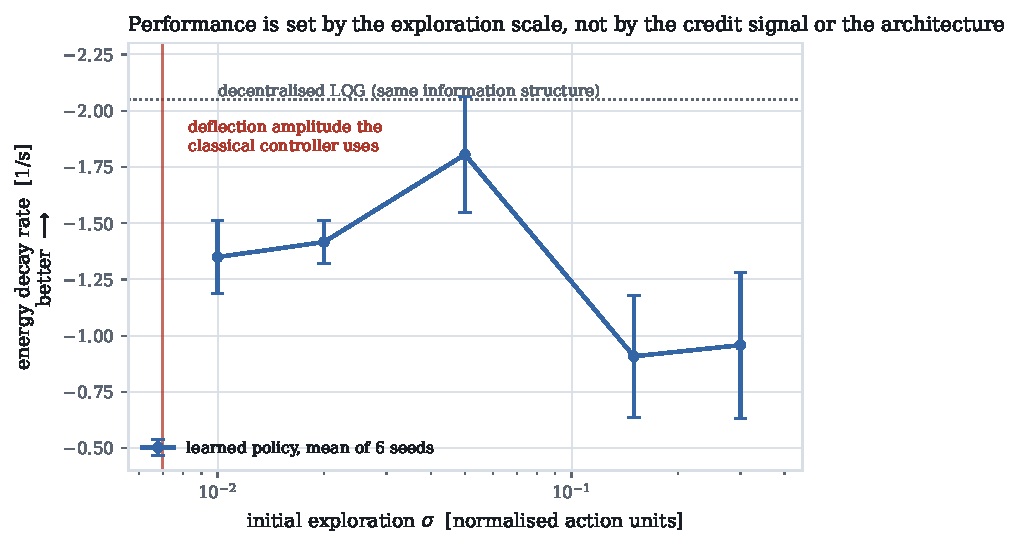
\includegraphics[width=0.8\textwidth]{figures/fig_exploration.pdf}
\caption{Decay rate against initial exploration standard deviation, all
else fixed. The vertical line marks the deflection amplitude the classical
controller uses. Six seeds per point.}
\label{fig:exploration}
\end{figure}

This is the finding with the widest reach. Holding everything else fixed
and varying only the initial exploration standard deviation moves
performance by a factor of two ($-1.805\pm0.257$ at $\sigma=0.05$ against
$-0.908\pm0.271$ at $\sigma=0.15$, a ratio of $1.99$), with an interior
optimum at $\sigma=0.05$. The mechanism reads off the axis: a controller
achieving the classical result uses about \SI{0.105}{\degree} RMS
deflection; $\sigma=0.30$ corresponds to \SI{4.5}{\degree} -- the policy's
own exploration is some forty times the amplitude that works, and no
credit decomposition can recover a signal buried underneath it. This is
not a tuning remark: before finding it, every variant plateaued between
$-0.03$ and $-0.82\,\mathrm{s}^{-1}$ regardless of credit signal,
communication, action parameterisation, memory, auxiliary supervision, or
base controller (six-seed variance details in the Supplemental Material,
Section S5). A capability probe rules out the competing explanation:
training on the single easiest condition gives $+0.21$ and $+0.27$, worse
than training on the full distribution, so the plateau was never a matter
of the task being too broad. The practical recommendation is specific: the
useful actuation amplitude is computable before any training, from a
classical design or an estimate of the damping authority required. Scale
the exploration to it; on this problem that single number mattered more
than every algorithmic choice we made, and it is cheap to check.

\subsection{Sensitivity to control-influence identification error}
\label{sec:credit-sensitivity}

The credit signal's sign is decided by the modal residue $v_r^{\top} b_k$,
free in simulation but requiring an identified control-influence estimate
on hardware; a wrong sign rewards a surface for exciting a mode rather
than damping it. Modelling identification error as an independent relative
perturbation on each entry of $B$, the most fragile surface--mode pairing
flips sign at just \SI{11}{\percent} relative error, essentially
speed-invariant across the flight envelope; every other entry tolerates
more, up to entries that do not flip within $\pm100\,\%$ error at all
(full per-entry results in the Supplemental Material, Section S6). Under a
\emph{uniform} per-surface scale error instead, every sign flips
simultaneously only at $-100\,\%$ (classical control reversal); the
plant's own $+90\,\%$ UVLM control-authority overestimate
(Section~\ref{sec:sharpy}) moves the assumed value \emph{away} from that
boundary, a safety factor of roughly $2$--$3\times$ in the direction that
already occurred. Retraining with the credit signal's belief about control
authority perturbed by a uniform $\pm\SI{60}{\percent}$ (three seeds) does
not collapse performance or reverse its sign in either direction
(Supplemental Material, Section S6): moderate uniform identification error
degrades gracefully rather than catastrophically, though we have not
tested past the $-100\,\%$ reversal boundary itself.

\section{Discussion and conclusion}
\label{sec:discussion}

This study set out to ask whether treating each control surface as a
separate learning agent is workable for flutter suppression, and the
answer is conditional. On credit assignment, yes, with numbers behind it:
a physics-derived signal, requiring no estimation step, is competitive
with the estimated alternatives we tested and more consistent across seeds
and conditions than any of them. On whether the resulting policies are
ready to fly, not yet -- the gap to a classical decentralised design on
average nominal damping is real rather than an artefact of tuning
(Section~\ref{sec:robust-baseline}), and the learned policies have no
certification pathway or stability-margin guarantee, unlike every
classical rung.

The most actionable finding for practitioners is the least glamorous one:
before training a policy for a physical control task, compute the
actuation amplitude a competent classical controller would use and check
the initial exploration scale against it. On this plant the two were
separated by a factor of forty at a conventional PPO setting, and every
algorithmic refinement we tried was invisible until that gap was closed;
we expect this check to be worth running on any task where a classical
baseline is available even loosely. Flutter suppression is
flight-safety-critical by construction, and nothing here argues the
learned policies as trained are ready for that role -- we place this work
at approximately TRL 2--3, a validated simulation testbed and a
first-principles credit signal with no wind-tunnel or hardware-in-the-loop
evidence yet. The residual formulation offers the most concrete path we
see toward certifiable: \texttt{residual\_only} is, by construction, a
certifiable decentralised LQG base law plus a learned correction
initialised near zero and bounded to a fixed authority fraction. A
run-time-assurance architecture on the same structure -- the certified law
as default, the correction bounded, and a monitor that reverts to the base
law outside a pre-verified envelope -- would let the learned component
fail safe into a controller already certifiable on its own; we have not
built or verified such a monitor, nor characterised how the credit
signal's identification-error robustness interacts with the monitor's
authority bound, and flag both as the concrete next step.

We did not expect the phasor consensus and phase-locked action head to
hurt. A plausible interpretation is that a three-surface, six-metre wing
with broadcast air data is too small a coordination problem for an
explicit channel to earn its bandwidth cost, and the eight-surface result
(Supplemental Material, Section S5) is at least consistent with that
story, though not run to the statistical standard we hold the main claims
to; we read this as a caution against building communication machinery
into a distributed controller by default, without first checking whether a
plain policy with the same credit signal already does the job. We still
find the phase-coordination result the most striking one: a policy trained
end to end on a shaped scalar reward, using only its own two
accelerometers, converges on the same resonant frequency that a
full-state, Kalman-filtered LQG converges on by construction -- a property
of the coupled structure the policy has to find, not supplied anywhere in
the reward, the observation, or the network architecture, which is the
sense in which we think ``emergent'' is earned here rather than merely
asserted.

\subsection{Limitations}
\label{sec:limitations}

\begin{itemize}
\item The learned policies do not match the decentralised classical
controller on average nominal damping ($-1.53$ against
$-2.05\,\mathrm{s}^{-1}$); they are more uniform across the envelope and
hold one condition it diverges on, but we do not claim they dominate it.
\item The robustness result is scale-dependent (Section~\ref{sec:results});
we report the trade-off rather than its better half.
\item The plant over-estimates control authority by $1.9\times$ relative to
UVLM (Section~\ref{sec:sharpy}); relative comparisons are unaffected but
absolute decay rates would not transfer, and we have not retrained on the
UVLM plant or characterised how the credit decomposition would degrade
under a higher-fidelity model with inter-surface aerodynamic coupling.
\item The credit signal requires a modal control-influence estimate that is
free in simulation but identified on hardware; the least robust
surface--mode pairing tolerates only \SI{11}{\percent} independent
relative error before its sign reverses (Section~\ref{sec:credit-sensitivity}),
though the plant's own measured discrepancy is well clear of that
boundary.
\item Ablations use six seeds on a three-surface wing; the eight-surface
results and three further probes (Supplemental Material, Section S5) are
one- and two-seed and not run to the same standard. Correcting for the
number of
comparisons made changed which credit comparisons are significant, and
bringing the exploration sweep to six seeds changed our estimate of its
seed-to-seed spread substantially, though not the qualitative shape of the
curve.
\item The exploration finding is established on this plant and algorithm;
we expect it to generalise to control tasks with a narrow useful actuation
band relative to the action range, but have not shown that.
\end{itemize}

\subsection{Conclusion}

Posing flutter suppression as a distributed learning problem exposes a
credit structure the physics resolves in closed form: the difference
reward is an agent's own control power, normalised by the instantaneous
energy so it coincides with the objective and cannot be gamed by
sustaining the oscillation. Combined with log-energy shaping it beats the
closed form used alone, once compared and corrected for multiple
comparisons against the full family of alternatives a reviewer would want
to see it measured against; against estimated credit signals, its
advantage is reliability across seeds and conditions rather than a
uniformly larger effect. The more transferable lesson is the caution: that
result, and a clean negative result on communication machinery, were both
invisible until the exploration scale was matched to the actuation
amplitude that damps the wing -- a quantity computable in advance from a
classical design, which mattered more here than any algorithmic choice we
made, and which we suspect is true of active vibration control more
broadly.

\section*{Funding Sources}
This work received no external funding or grant support.

\section*{Data and Code Availability}
The plant, baselines, training code, evaluation harness, and the SHARPy
cross-validation and sensitivity-analysis scripts referenced throughout
this paper and its Supplemental Material are available at the project
repository.

\section*{Acknowledgments}
The author declares no known competing financial interests or personal
relationships that could have appeared to influence the work reported in
this paper. Generative AI tools (Claude, Anthropic) were used during this
work to assist with software development, data-analysis scripting, and
manuscript preparation and editing. All AI-assisted code, analysis, and
text were reviewed and verified by the author, who takes full
responsibility for the content of this publication.

\bibliography{refs,refs_extra}

\end{document}
